\documentclass[final]{pittetd}
%
\usepackage[%
    backend    = biber,%
    style      = chem-acs,%
    autocite   = superscript,%
    backref    = true,%
    biblabel   = brackets,%
    doi        = true,%
    minnames   = 1,%
    maxnames   = 999,%
]{biblatex}
\DefineBibliographyStrings{english}{%
  backrefpage = {page},% originally "cit. on p."
  backrefpages = {pages},%
}
\addbibresource{./example.bib}
%
\usepackage{algorithm}
\usepackage{algpseudocode}
\usepackage{booktabs}
\usepackage{etoolbox}
\usepackage{graphicx}
\usepackage[usenames,dvipsnames,svgnames,hyperref,table]{xcolor}
%
\BeforeBeginEnvironment{algorithmic}{\begin{singlespace}}
\AfterEndEnvironment{algorithmic}{\end{singlespace}}
%
\definecolor{carmine}{HTML}{960018}
%
\hypersetup{%
  colorlinks=true,%
  citecolor=black,%
  linkcolor=black,%
  urlcolor=carmine,%
}
%
% First-principles decomposition of spectroscopic response
\title{Decomposition of Intermolecular Interactions in \textit{ab initio} Spectroscopy}
\author{Eric John Berquist}
\degree{B.S. Chemistry, Northeastern University, 2012}
\keywords{ionic liquids, carbon dioxide, infrared spectroscopy, energy decomposition analysis, absolutely localized molecular orbitals, polarizability, linear response}
\subject{First-Principles Computational Decomposition of Spectroscopic Response}
\school[the Kenneth P.\ Dietrich School of]{Arts and Sciences}
\setyear{2018}
\date{March 23rd, 2018}
\committeemember{Daniel S. Lambrecht, Assistant Professor, Department of Chemistry}
\committeemember{Kenneth D. Jordan, Professor, Department of Chemistry}
\committeemember{Sean Garrett-Roe, Assistant Professor, Department of Chemistry}
\committeemember{David Yaron, Professor, Department of Chemistry, Carnegie Mellon University}
\school{Kenneth P.\ Dietrich School of Arts and Sciences}

\begin{document}
\maketitle
\makecommittee
\copyrightpage
\begin{abstract}
  I am a short stub abstract.
\end{abstract}

\tableofcontents
\listoftables
\listoffigures
%
\preface
I am the preface contents. Please write me last.

%
\newcommand{\op}[1]{\ensuremath{\hat{#1}}}
\newcommand{\lr}[2]{\braket{\braket{\op{#1}; \op{#2}}}}
\newcommand{\mat}[1]{\ensuremath{\mathbf{#1}}}
\newcommand\qchem{\textsc{Q-Chem}}

\chapter{First chapter}

I am fake contents of the first chapter.

\section{First section}

I am the first section.

\begin{figure}
  \centering
  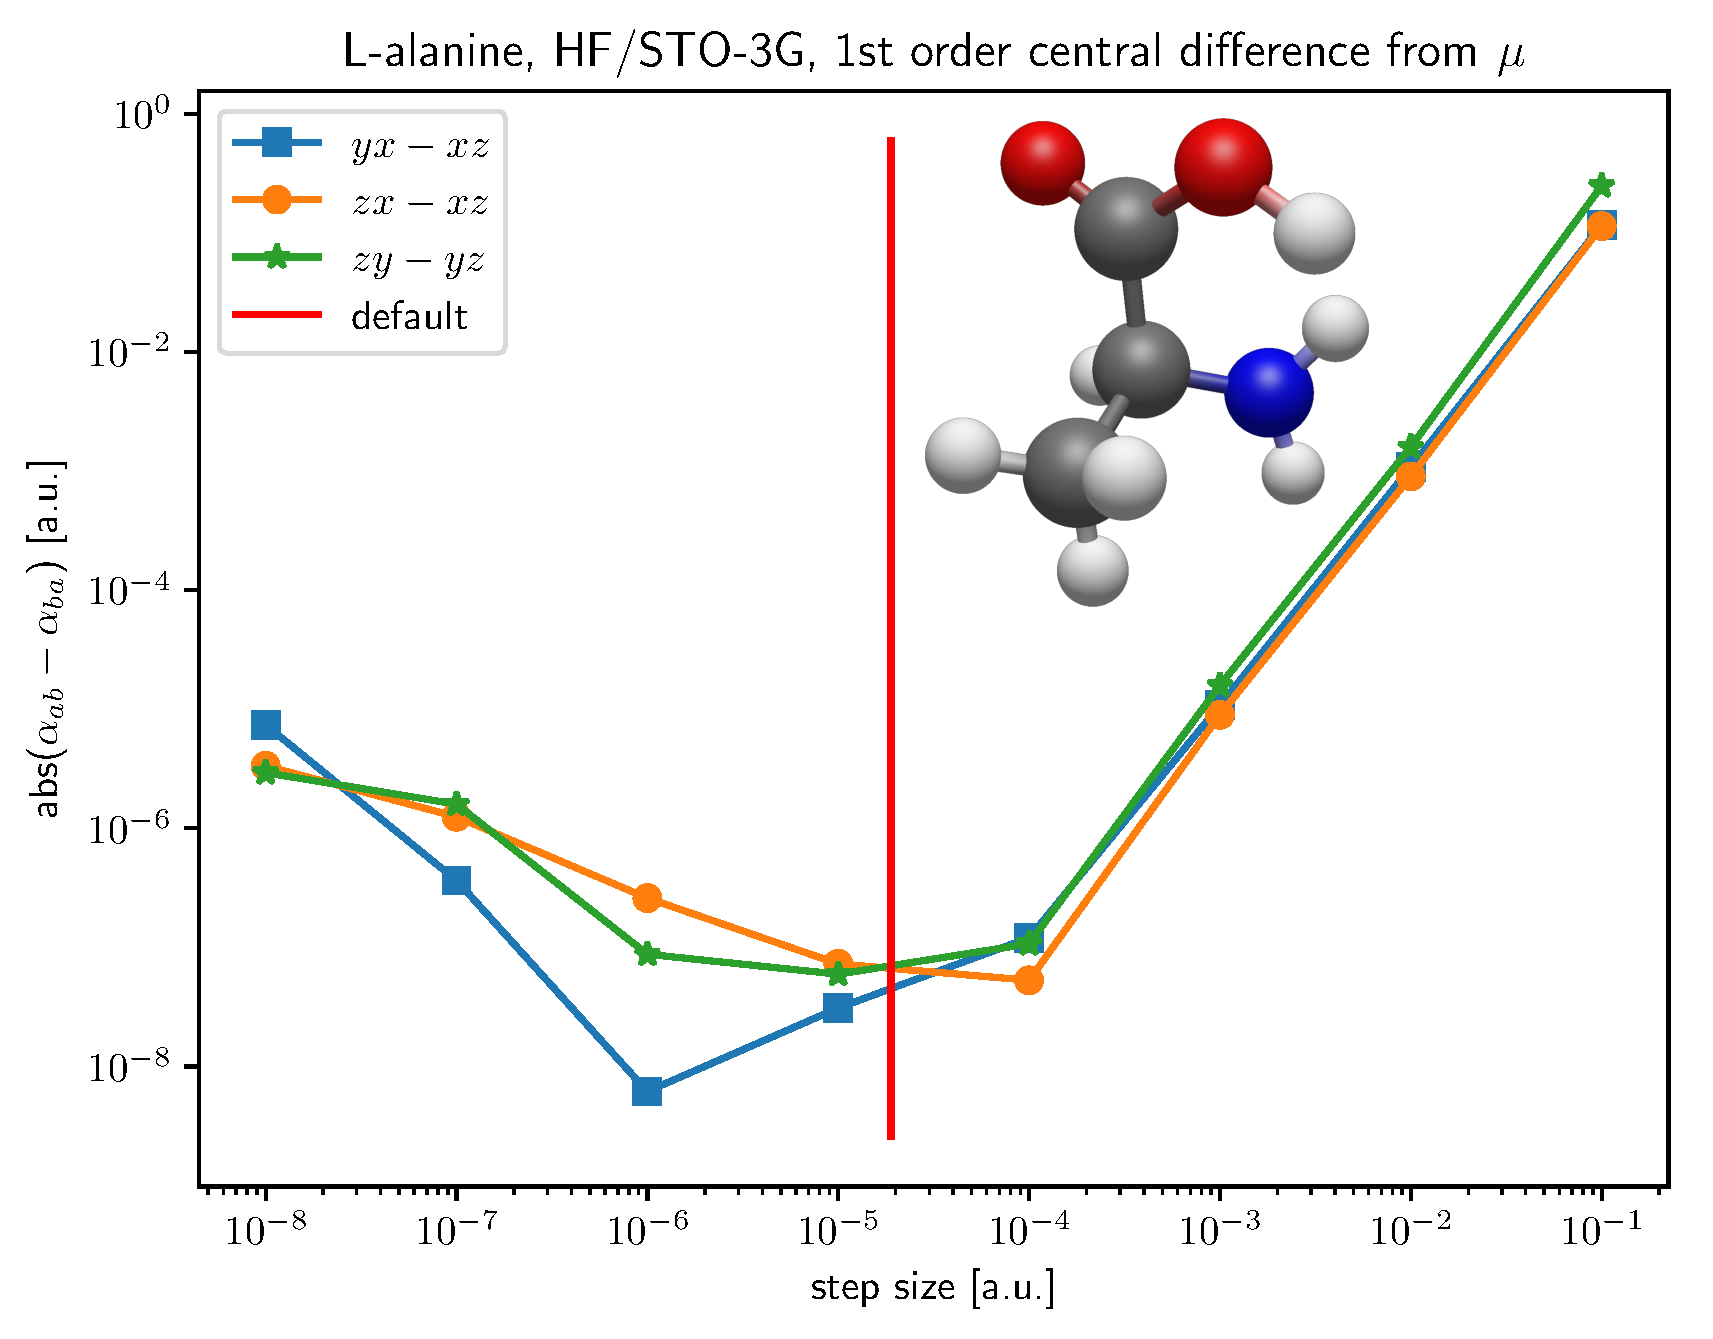
\includegraphics[width=0.90\textwidth]{./diff_overlay.pdf}
  \caption{Asymmetry in the 1st-order finite-difference polarizability\label{fig:finite-difference-numerical-noise}}
\end{figure}

\begin{table}
  \centering
  \caption[MO coefficient derivatives and rotation matrices needed for energy derivatives]{Orders of MO coefficient derivatives and rotation matrices needed for energy derivatives following Wigner's \(2n+1\) rule. Reproduced from Ref.~\parencite{Yamaguchi1994}.\label{tutorial:tab:wigner}}
  \begin{tabular}{cccc}
    \toprule
    & CI: MO/CI space & MCSCF: MO/CI space & RHF: MO space \\
    \midrule
    Energy, \(E\) & \(C_{\mu}^{i}\), \(C_{I}\) & \(C_{\mu}^{i}\), \(C_{I}\) & \(C_{\mu}^{i}\) \\
    First Derivative, \(\frac{\partial E}{\partial a}\) & \(U^{a}\), \(C_{I}\) & \(C_{\mu}^{i}\), \(C_{I}\) & \(C_{\mu}^{i}\) \\
    Second Derivative, \(\frac{\partial^{2} E}{\partial a \partial b}\) & \(U^{ab}\), \(\frac{\partial C_{I}}{\partial a}\) & \(U^{a}\), \(\frac{\partial C_{I}}{\partial a}\) & \(U^{a}\) \\
    Third Derivative, \(\frac{\partial^{3} E}{\partial a \partial b \partial c}\) & \(U^{abc}\), \(\frac{\partial C_{I}}{\partial a}\) & \(U^{a}\), \(\frac{\partial C_{I}}{\partial a}\) & \(U^{a}\) \\
    Fourth Derivative, \(\frac{\partial^{4} E}{\partial a \partial b \partial c \partial d}\) & \(U^{abcd}\), \(\frac{\partial^{2} C_{I}}{\partial a \partial b}\) & \(U^{ab}\), \(\frac{\partial^{2} C_{I}}{\partial a \partial b}\) & \(U^{ab}\) \\
    Fifth Derivative, \(\frac{\partial^{5} E}{\partial a \partial b \partial c \partial d \partial e}\) & \(U^{abcde}\), \(\frac{\partial^{2} C_{I}}{\partial a \partial b}\) & \(U^{ab}\), \(\frac{\partial^{2} C_{I}}{\partial a \partial b}\) & \(U^{ab}\) \\
    \bottomrule
  \end{tabular}
\end{table}

\begin{algorithm}
  \(i,j\) are input/output node indices into the weight coefficient matrix.
  \begin{algorithmic}[1]
    \State Training set \(\gets \{ (x^{(1)},y^{(1)}), ..., (x^{(m)},y^{(m)}) \}\)
    \State \(\Delta_{ij}^{(l)} \gets 0\) for all \(l,i,j\)
    \For{training example \(t \gets 1, m\)}
      \State \(a^{(1)} \gets x^{(t)}\)
      \State Perform forward propagation to compute \(a^{(l)}\) for \(l=2,3,...,L\)
      \State \(\delta^{(L)} \gets a^{(L)} - y^{(t)}\)
      \Comment{Initialize backpropagation routine at output layer.}
      \For{\(l \gets L-2, 2\)}
        \Comment{Work backwards through layers.}
        \State \( g'(s^{(l)}) \gets a^{(l)} \odot (1 - a^{(l)}) \)
        \State \( \delta^{(l)} \gets ( (w^{(l)})^{T} \delta^{(l+1)} ) \odot g'(s^{(l)}) \)
        %% \State \( \Delta_{ij}^{(l)} \gets \Delta_{ij}^{(l)} + a_{j}^{(l)} \delta_{i}^{(l+1)} \) for all \(i,j\)
        \State \( \Delta^{(l)} \gets \Delta^{(l)} + \delta^{(l+1)} (a^{(l)})^{T}  \)
        \State \(D_{ij}^{(l)} \gets \frac{1}{m} \Delta_{ij}^{(l)} + \lambda w_{ij}^{(l)} \)
      \EndFor
    \EndFor
    \State \( \frac{\partial}{\partial w_{ij}^{(l)}} J(w) \gets D_{ij}^{(l)} \)
  \end{algorithmic}
  The regularization term with hyperparameter \(\lambda\) is set to zero if \(j = 0\) (the bias node).
  \caption{Backpropagation for computing weight updates in a fully-connected neural network}
\end{algorithm}

\algnewcommand\Break{\textbf{break}}
\algnewcommand\Not{\textbf{not}}
\algnewcommand\True{\textbf{true}}
\algnewcommand\False{\textbf{false}}
\algnewcommand\Rhsvecs{\textsf{rhsvecs}}
\algnewcommand\Rspvecs{\textsf{rspvecs}}
\algnewcommand\Operators{\textsf{operators}}
\algnewcommand\Resp{\textsf{resp}}
\algnewcommand\AllowCT{\textsf{allow\_ct?}}

\begin{algorithm}
  \centering
  \begin{algorithmic}[1]
  \Procedure{solve\_linear\_response}{\Resp, \Operators, occupations, \(\mat{C}, \mat{F}, \mat{S}, \vartheta\), maxiter, \AllowCT}
  \For{\(s \gets 1, N_{spin}\)}
    \State Transformation of \(\mat{F}\) and \(\mat{S}\) from AO to full MO basis
    \State \(E_{ia,jb} = F_{ab}S_{ij} - F_{ij}S_{ab}\)
    \Comment{Form non-orthogonal orbital energy matrix \(\mat{E}\)}
    \If{\Not{} \AllowCT{}}
      \State Zero cross-fragment \(ia\) indices and shrink dimensions of \(\mat{E}\)
    \EndIf
    \State Form inverse for denominator \(\mat{E}^{-1}\)
  \EndFor
  \For{\(i \gets 1, N_{operators}\)}
    \For{\(c \gets 1, N_{components}\)}
      \State \((\mat{Z})_{\mu\nu} \gets \Operators[i,c,\mu\nu]\)
      \Comment{Select operator component as perturbation for right-hand side}
      \State Transform operator component from AO to occ-virt MO basis and append \(\mat{Z}_{ia}\) to \Rhsvecs
      \If{\Not{} \AllowCT{}}
        \State Zero cross-fragment \(ia\) indices and shrink dimensions of \(\mat{Z}\)
      \EndIf
      \State \(\mat{X}^{(0)} \gets \mat{0}\)
      \Comment{Form initial guess for response vector (uncoupled result)}
      \State \(converged \gets \False\)
      \For{\(n \gets 1, maxiter\)}
        \State \(D_{\mu\nu}^{X} \gets C_{\mu i} X_{ia}^{(n-1)} C_{\nu a}\)
        \Comment{Form perturbed density}
        \State \(J_{\mu\nu}^{X}\left[\mat{D}^{X}\right], K_{\mu\nu}^{X}\left[\mat{D}^{X}\right] \gets fock\_build(\mat{D}^{X})\)
        \Comment{Form Coulomb and exchange contributions}
        \State \(\left(\mat{R}^{(n)}\right)_{\mu\nu} \gets 4 \mat{J}^{X} - \mat{K}^{X} - \left(\mat{K}^{X}\right)^{T}\)
        \Comment{Form half-transformed orbital Hessian-vector product (here, \(\mat{G} = \mat{A}^{s} + \mat{B}^{s}\))}
        \State Do second transformation of Hessian-vector product \(\left(\mat{R}\right)_{ia}^{(n)}\)
        \If{\Not{} \AllowCT{}}
          \State Zero cross-fragment \(ia\) indices and shrink dimensions of \(\mat{R}, \mat{X}\)
        \EndIf
        \State \(X_{ia}^{(n)} \gets (\mat{E}^{-1})_{ia,jb} \left[ Z_{jb} - R_{jb}^{(n)} \right]\)
        \Comment{Update response vector}
        \If{\Not{} \AllowCT{}}
          \State Restore dimensions of \(\mat{X}\)
        \EndIf
        \If{\(||\mat{X}^{(n)} - \mat{X}^{(n-1)}|| < \vartheta\)}
          \State \(converged \gets \True\)
          \State Append \(\mat{X}^{(n)}\) to \Rspvecs
          \State \Break
        \EndIf
  \algstore{lrmi}
  \end{algorithmic}
  \caption{Static linear response approach within fragment-localized formalism.\label{alg:solve-linear-response}}
\end{algorithm}
\begin{algorithm}
  \centering
  \begin{algorithmic}[1]
  \algrestore{lrmi}
        \EndFor
      \If{\Not{} \(converged\)}
        \State crash
      \EndIf
    \EndFor
  \EndFor
  \State \(\Resp \gets \mat{0}\)
  \Comment{Form all possible permutations of property gradient and response vectors}
  \For{\(a \gets 1, len(\Rhsvecs)\)}
    \For{\(b \gets 1, len(\Rspvecs)\)}
      \State \(\mat{P} \gets \Rhsvecs[a], \mat{Q} \gets \Rspvecs[b]\)
      \State \(\lr{P}{Q}_{0} \gets -P_{ia}Q_{ia}\)
      \State \(\Resp[a,b] \gets \lr{P}{Q}_{0}\)
    \EndFor
  \EndFor
  \EndProcedure
  \end{algorithmic}
  \caption{Continuation of algorithm~\ref{alg:solve-linear-response}\label{alg:solve-linear-response-2}}
\end{algorithm}

\begin{lstlisting}[%
  frame=single,%
  label=listing:input-almo-eda-gen1,%
  caption=Sample \qchem{} input file for first-generation ALMO-EDA. Geometry is from HF/def2-SVPD.%
]
$rem
  jobtype = eda
  method = hf
  basis = def2-svpd
  scf_convergence = 11
  thresh = 14
  scf_max_cycles = 1000
  symmetry = false
  sym_ignore = true
  cc_symmetry = false
  scf_print_frgm = false
  frgm_method = stoll
  frgm_lpcorr = rs_exact_scf
  eda_bsse = true
$end

$molecule
1 1
--
0 1
Ar     0.000000000000000    0.000000000000000   -0.857713330500000
--
1 1
Li     0.000000000000000    0.000000000000000    1.571999044800000
$end
\end{lstlisting}

%
\printbibliography[title=BIBLIOGRAPHY]
%
\end{document}
